\subsection{Judas}

Judas, formerly known as Emerald \cite{projthesis}, is a Julia package we've created for internal use for members at \acrshort{cgf}. Our work started last fall, when we saw a limitation of current applications at \acrshort{cgf} for loading \acrshort{das} data from local servers into programs to be able to process and further analyze these data. We chose to write this package in Julia both due to its high performance, and members' familiarity with similar languages such as MatLab and Python. With Julia, we could draw strengths from its ecosystem and build systems to create an easy-to-use library for members to familiarize themselves with. We did so by starting off with a simple python program, that read multiple \acrshort{hdf5} files storing \acrshort{das} data into dataframes. From here, we parallellized certain parts of the code, and opted to store processed data in memory mapped files instead of loading large matrices into memory. This allowed us to work with more data at the same time, as well as decreasing the overall wall time and memory consumption.  

In this section, we will be looking at what changes has been made ever since, from improvements of existent code, to new methods added and the availability of the library for members at \acrshort{cgf}. \\

Following our previous work, we will be working with data recorded from BANENOR, specifically a train route between Trondheim and Storen with recorded values from the 31st of August 2021 \footnote{Working with national infrastructure requires security clearance, see \ref{app:conf} for more details}. 

\begin{table}[h]
    \centering
    \begin{tabular}{|l|l|}
        \hline
        \textbf{Parameter} & \textbf{Value} \\
        \hline
        Experiment & 210830\_NTNU\_Bane\_NOR\_GL8De4F2000 \\
        \hline
        File timestamp & 2021-08-31 10:00:01 \\
        \hline
        Type of data & Phase rate per distance, unit: rad/m/s \\
        \hline
        Sampling frequency & 2000.0 Hz \\
        \hline
        Distance between channels & 4.0852 m \\
        \hline
        Data shape & 20000 samples x 12500 channels \\
        \hline
        Gauge length & 8.170401526197452 m \\
        \hline
        Sensitivities & 9.362208901094029e6 r \\
        \hline
        Regions of interest & 1:4:49996 \\
        \hline
    \end{tabular}
    \caption{BANENOR Experiment Data Summary}
    \label{tab:experiment_data}
\end{table}

As we can see in table \ref{tab:experiment_data}, the total distance of this dataset is approximately 50km, where we have stored data for every 4th sensor across the route. Each file contains 10 seconds of data, leading us to get a matrix of size $20000 x 12500$, where each element is of type \texttt{Float32}, giving us a total of 8GB to be stored for every 10 seconds. This obviously is challenging to work with, so we will go further in depth on how we use resampling and channel decimation to be able to reduce memory usage yet still retain the most important aspects of our signal data. \\

\begin{table}[h]
\centering
\begin{tabular}{|r|r|r|r|r|}
\hline
\textbf{1}                & \textbf{2}               & \multicolumn{1}{c|}{\textbf{...}} & \textbf{n-1}             & \textbf{n}               \\ \hline
1f-3                      & 2.3f-5                   & 4f-4                              & 3.4f-6                   & 3f-1                     \\ \hline
3f-1                      & 3f-1                     & 3f-1                              & 3f-1                     & 3f-1                     \\ \hline
\multicolumn{1}{|c|}{...} & \multicolumn{1}{c|}{...} & \multicolumn{1}{c|}{...}          & \multicolumn{1}{c|}{...} & \multicolumn{1}{c|}{...} \\ \hline
4f-2                      & 3f-1                     & 3f-1                              & 3f-1                     & 3f-1                     \\ \hline
\end{tabular}
\caption{Table showcasing how \acrshort{das} data is stored in matrices with $n$ channels and $t$ timestamps}
\label{fig:datatable}
\end{table}

To best showcase what changes and improvements have been made, \ref{fig:apiflow} visualizes the order of high level operations to done on our data. In addition, we will be demonstrating mostly the new additions to the code, as well as the changes to the loading and preprocessing of the data. \\

\begin{figure}[h]
    \centering
    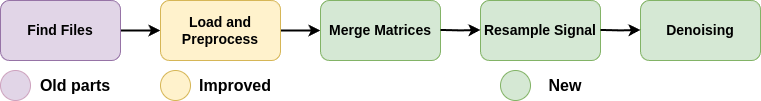
\includegraphics[scale=0.5]{figures/dataflow.png}
    \caption{Dataflow from we read HDF5 files to we are ready to train}
    \label{fig:apiflow}
\end{figure}

The DAS folder has not changed much substantially. The main difference from before is how we now instead of writing matrix data to one large binary file, data is split into multiple files, and only read when needed.

Contrary to what was mentioned before, the output of the function \texttt{load\_DAS\_files} has actually changed. Previously, we stored a whole vector of the timestamps for each sample. Not only was this cistly, but actaully totally redundant. If the timestamp of the first row is known, the sampling rate $T$ and which row to look at, one can instead calculate the timestamp like this: 
\lstinline|start_time + MilliSecond(idx * T * 1000)|. This in-place calculation can be done multiple times effectively in Julia using the broadcast operator (.). This ensures that we don't lose essential information before running our data through through the autoencoder

\begin{figure}[h]
\centering
\begin{subfigure}{.45\textwidth}
  \centering
  \lstinputlisting[language=Julia]{code/dasstructold.jl}
  \caption{Old DAS Struct}
  \label{fig:olddasstc}
\end{subfigure}%
\hfill
\begin{subfigure}{.45\textwidth}
  \centering
  \lstinputlisting[language=Julia]{code/dasstruct.jl}
  \caption{New Layout for DAS struct}
  \label{fig:newdasstc}
\end{subfigure}
\caption{Comparison between different versions of the DAS struct}
\label{fig:dasstccmp}
\end{figure}



\textbf{API Usage}

\begin{figure}[h]
    \centering
    \lstinputlisting[language=Julia]{code/judas_usage.jl}
    \caption{How to use our API}
    \label{fig:apiusage}
\end{figure}


\begin{figure}[h]
    \centering
    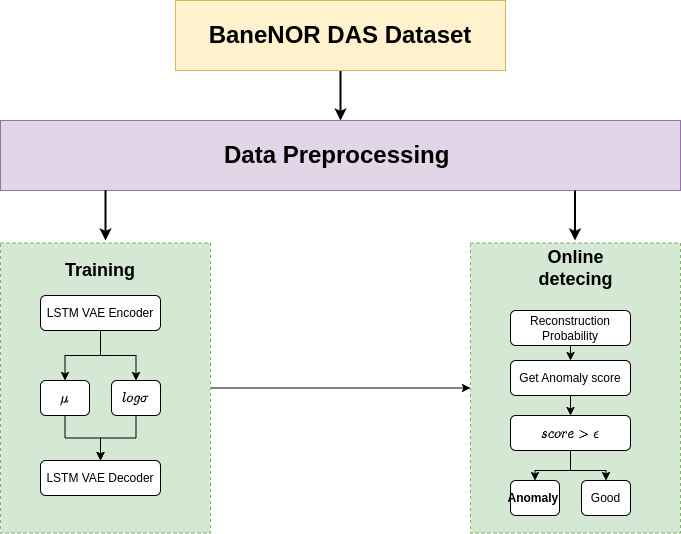
\includegraphics[scale=0.5]{figures/methodflow.png}
    \caption{Dataflow}
    \label{fig:dataflow}
\end{figure}
 
We start at the same spot we left off after the project thesis. Before we go on to explain what's been done this semester, lets recap. 

We initially got started by just getting a drive with lots of \acrshort{das} data, and a script from \acrfull{asn} which set up us perfectly. We chose to rewrite python code to a language similar to that of Matlab and Python. We landed on Julia, and with its broad ecosytstem it has support for all kinds of development we'd ever need. \\

We first wrote a 1:1 copy of the script, and then parallelized parts of the code until we had a version that could handle large amounts of data in parallel. We also wrote methods for being able to run a window over and \\ 


\section{Overview}

Our product is split into two apis. Those being \texttt{Judas} and \texttt{JudasNET}. Judas is the direct continuation from \cite{projthesis}
The \acrshort{api} that's being created is called \texttt{Judas} (Julia and DAS) and is split in 3 modules as well as a seperate Utils file as shown in \ref{fig:ccuda}

\begin{figure}[h]
    \centering
    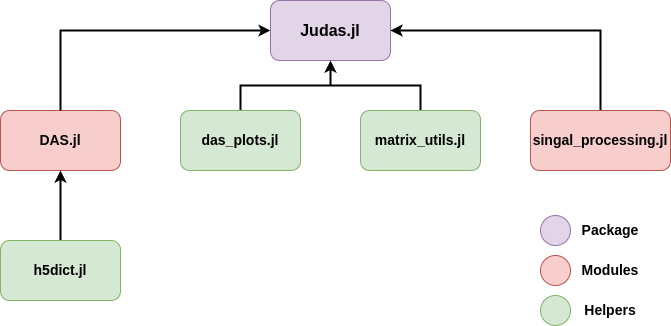
\includegraphics[scale=.6]{figures/judas_overview.png}
    \caption{Overview over our package Judas}
    \label{fig:judasoverview}
\end{figure}



\section{SignalProcessing.jl}

After data has been read and processed, it's ready to be processed by signal processing functions 


\subsection{Pre processing}

\subsubsection{Resampling and Channel decimation}

Following our previous work \cite{projthesis}, the following improvements have been made to \texttt{Judas}: 

\begin{enumerate}
    \item Judas now make use of multiple processors contra multithreading, seeing major speedups.
    \item Function \texttt{load\_DAS\_files} now writes processed data to a single file back.
    \item Methods for resampling and chann
\end{enumerate}


\subsubsection{Window and Filter operations}

After the data has been loaded \cite{projthesis}, it's still not ready for processing. 

The function \lstinline|process_DAS_data| takes in the signal data, perform a tukey \ref{dsp:tukey} window algorithm over it. We then run a band-pass filter algorithm with Butterworth over it to extract the and 

\begin{figure}[h]
    \centering
    \lstinputlisting[language=Julia]{code/denoise.jl}
    \caption{Window and Filter operations of our \acrshort{das} data.}
    \label{fig:procdasdata}
\end{figure}


After applying a window function and a filter function to combat oscilleration, we're now ready to run an fft over this data. 





\begin{figure}[h]
    \centering
    \lstinputlisting[language=Julia]{code/judas_usage.jl}
    \caption{Flux normalization function}
    \label{fig:judas_usage}
\end{figure}
